\section{Introduction}

Masked Diffusion Models (MDMs) have emerged as a powerful alternative to the dominant autoregressive paradigm for discrete sequence generation~\cite{austin2021structured, lou2024discrete,nie2025large}. By leveraging bidirectional attention, MDMs break free from strict left-to-right generation, granting unprecedented flexibility in decoding paths~\cite{rombach2022high}. This flexibility unlocks superior performance in tasks requiring bidirectional attention, such as code infilling, biological sequence design, and long-horizon planning tasks~\cite{ye2025dream, gong2024scaling,ye2024beyond}.

However, this potential remains largely untapped due to a training--inference mismatch. While MDMs are trained under random masking patterns, inference entails a multi-step, order-sensitive decoding process. Navigating the large space of possible decoding orders therefore requires a sampler that carefully selects which tokens to reveal next. Consequently, generation quality is heavily dependent on the effectiveness of the sampler~\cite{kim2025train}.

Existing samplers predominantly rely on \textbf{local certainty heuristics} such as confidence to greedily select the next decoding target~\cite{chang2022maskgit, ye2025dream, huang2025pc, kim2025train}. In Section~\ref{sec:motivation}, we argue and demonstrate that such samplers are often nonrobust due to the myopia of local heuristics: they ignore the long-term impact of current decoding decisions on future uncertainty. Consequently, they frequently prioritize tokens that appear syntactically \textit{confident} but are semantically suboptimal, leading to error propagation and compromised generation quality.


In contrast to autoregressive models (ARMs), where the causal nature makes evaluating the downstream effect of a token choice computationally prohibitive, the bidirectional nature of MDMs offers a distinct advantage: it enables us to assess how a token decoding decision influences the uncertainty across all remaining masked positions immediately.

Leveraging these insights, we propose the \textbf{Information Gain (Info-Gain) Sampler}, a decoding framework that departs from greedy certainty-based sampling. Instead of merely refining the certainty scoring function, the Info-Gain Sampler additionally evaluates decoding actions by how much they reduce the uncertainty in remaining masked tokens. By balancing \textit{immediate certainty} with \textit{information gain}, our method prioritizes globally informative decisions and yields more robust decoding trajectories. Our contributions are threefold:

\begin{figure*}[t]
    \centering
    \begin{minipage}[t]{0.49\textwidth}
        \centering
        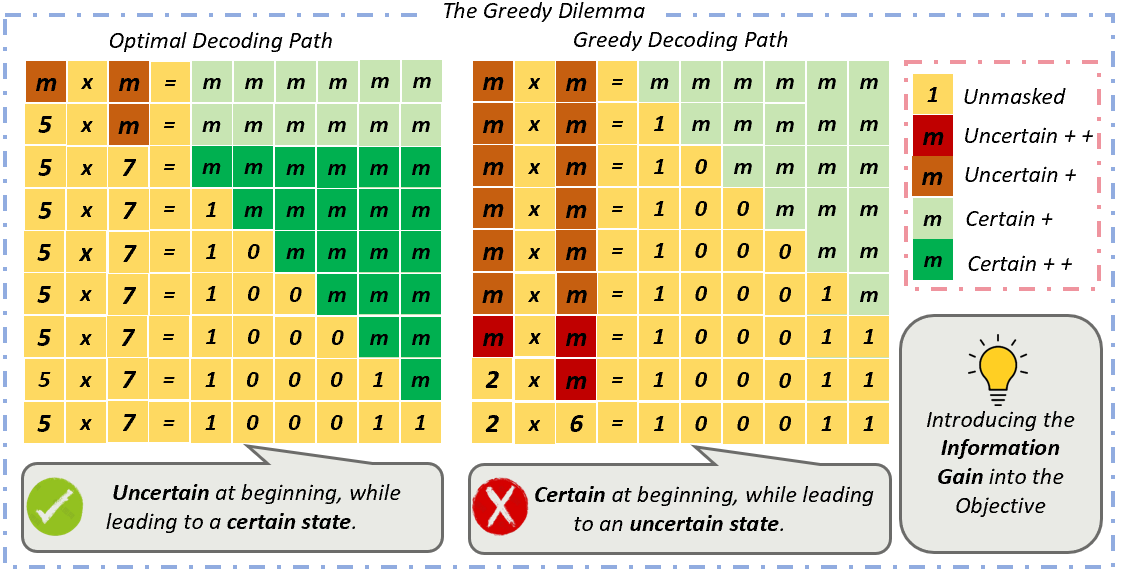
\includegraphics[width=\linewidth]{illustrative.png}
        \caption*{(a) The dilemma of greedy certainty-based sampling.}
        \label{fig:motivation}
    \end{minipage}
    \hfill
    \begin{minipage}[t]{0.49\textwidth}
        \centering
        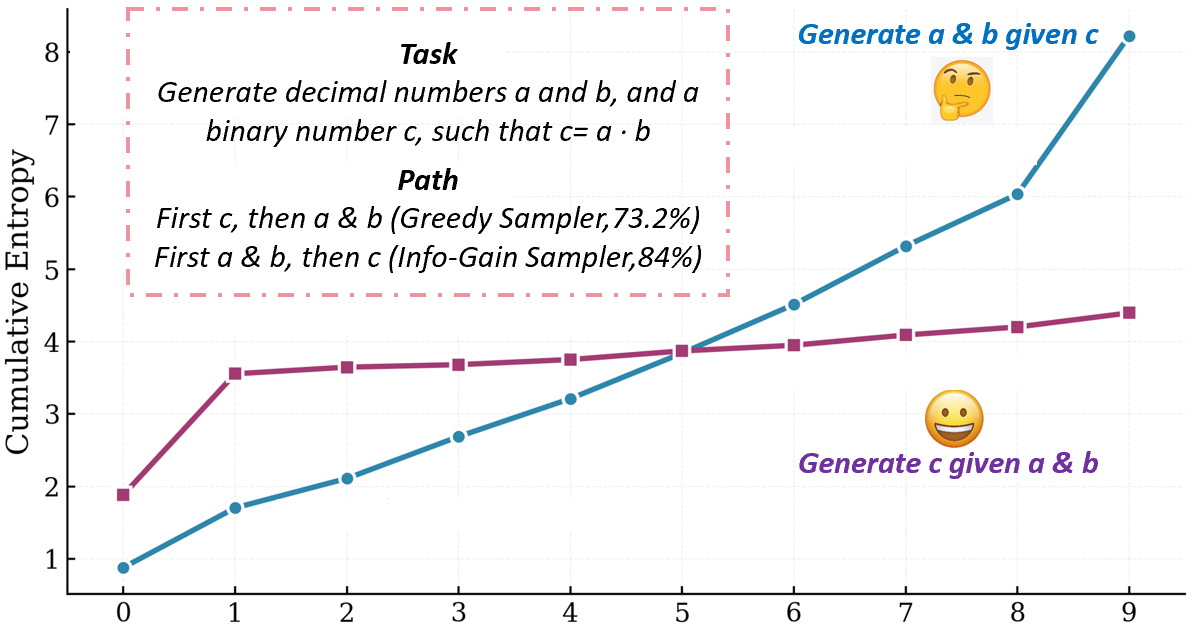
\includegraphics[width=\linewidth]{toy1-v4.png}
        \caption*{(b) Evolution of cumulative uncertainty.}
        \label{fig:toy_one_way}
    \end{minipage}

    \caption{
    \textbf{Motivation:} Analysis of decoding strategies on the one-way multiplication experiment.
    (a) Illustrates the contrast between the suboptimal path chosen by the greedy certainty-based sampler and the optimal path, motivating the introduction of the Info-Gain Sampler.
    (b) Shows the evolution of cumulative uncertainty throughout the decoding process.
    While the greedy sampler prioritizes decoding $c$ first (73.2\%) due to its immediate high confidence, it leads to failure because of the task's one-way nature.
    In contrast, the Info-Gain Sampler optimizes global uncertainty by resolving high-entropy factors $a$ or $b$ first (84.0\%), ensuring a successful decoding trajectory.
    }
    \label{fig:toy_analysis}
\end{figure*}


{(1) }We empirically identify the fundamental limitations of existing greedy certainty-based samplers in MDMs through failure case analyses.

{(2) }We introduce the Info-Gain Sampler, which balances immediate costs with future information gain via a simple yet effective objective. We also propose computationally efficient implementations of Info-Gain Sampler.

{(3) }We extensively evaluate Info-Gain Sampler against other sampler baselines across diverse pretrained MDMs and benchmarks. The results show that Info-Gain consistently outperforms these baselines across math, coding, planning, writing, and image generation tasks.
